\documentclass{endm}
\usepackage{endmmacro}
\usepackage{graphicx}
\usepackage{amsmath}

% The following is enclosed to allow easy detection of differences in
% ascii coding.
% Upper-case    A B C D E F G H I J K L M N O P Q R S T U V W X Y Z
% Lower-case    a b c d e f g h i j k l m n o p q r s t u v w x y z
% Digits        0 1 2 3 4 5 6 7 8 9
% Exclamation   !           Double quote "          Hash (number) #
% Dollar        $           Percent      %          Ampersand     &
% Acute accent  '           Left paren   (          Right paren   )
% Asterisk      *           Plus         +          Comma         ,
% Minus         -           Point        .          Solidus       /
% Colon         :           Semicolon    ;          Less than     <
% Equals        =           Greater than >          Question mark ?
% At            @           Left bracket [          Backslash     \
% Right bracket ]           Circumflex   ^          Underscore    _
% Grave accent  `           Left brace   {          Vertical bar  |
% Right brace   }           Tilde        ~

\newcommand{\Nat}{{\mathbb N}}
\newcommand{\Real}{{\mathbb R}}
\def\lastname{Brito}

\begin{document}  

% DO NOT REMOVE: Creates space for Elsevier logo, ScienceDirect logo
% and ENDM logo
\begin{verbatim}\end{verbatim}\vspace{2.5cm}

\begin{frontmatter}

\title{Creation of Conflict Graphs for Integer Programming: a Computational Study}

\author{Samuel Souza Brito\thanksref{myemail} \and Haroldo Gambini Santos\thanksref{coemail}}
 
\address{Computing Department\\ Universidade Federal de Ouro Preto - UFOP\\ Ouro Preto, Brazil}
\thanks[myemail]{Email:
   \href{mailto:samuelsouza@iceb.ufop.br} {\texttt{\normalshape
   samuelsouza@iceb.ufop.br}}} \thanks[coemail]{Email:
   \href{mailto:haroldo@iceb.ufop.br} {\texttt{\normalshape
   haroldo@iceb.ufop.br}}}

\begin{abstract}
This is a short example to show the basics of using the ENDM style
macro files. Ample examples of how files should look may be found
among the published volumes of the series at the ENDM home page
({\texttt{http://www.elsevier.com/locate/endm}})
\end{abstract}

\begin{keyword}
Please list keywords for your paper here, separated by commas.
\end{keyword}

\end{frontmatter}


\section{Introduction}\label{intro}

In this work we present an approach for the creation of conflict graphs for Integer Programming (IP) problems. A conflict graph represents logical relations between binary variables. This kind of graph has a vertex for each binary variable and its complement. An edge between two vertices indicates that the variables involved cannot be set to some specific value at the same time without violating some constraint of the problem.

Conflict graphs are typically constructed using probing techniques \cite{Borndorfer1998} based on constraints analysis. The probing technique consists in analyzing logical implications generated by fixing binary variables. For example, in a given problem the activation of the variable $x$ implies the deactivation (i.e. activation of its complement) of the variable $y$, in order to respect the constraints of the problem. In this case, we found a logical relation of the form ``$x = 1 \ \Rightarrow \ y = 0$''. This logical relation can be represented in a conflict graph, creating an edge between the vertice associated with $x$ and the vertice associated with $y$.


Building a graph by looking for pairwise of conflicts may be computationally prohibitive when the input problem is large. Thus, the computational efficiency of this technique depends on the complexity of the constraint exploration, causing a trade off between efficiency and effectivity. We also use probing techniques based on feasibility considerations, by analyzing constraint-by-constraint. However, we sort the coefficients and compute the bounds of the left-hand side for each constraint and compare with the respective right-hand side, in order to detect constraints that form cliques, avoiding the pairwise analysis of the variables in these constraints. The use of such strategy contributes to accelerate the conflict discovery process as shown in the performed experiments.

An important application for the use of conflict graphs is the clique cut generation, which performs a crucial role in the discovery of strong inequalities \cite{chvatal} in IP problems. The dynamic inclusion of these inequalities allows tightening the linear relaxation of an IP problem, crucial to the branch-and-bound based solvers \cite{atamturk}. Moreover, conflict graph can also be used to develop heuristics and branching primal schemes. Hoffman and Padberg \cite{hoffman} used conflict graphs to generate valid inequalities for set partitioning problems arising in airline crew-scheduling. Achterberg \cite{achterberg} presented heuristics based on SAT techniques for Mixed Integer Programming solvers to generate valid inequalities from the current infeasible subproblem and the associated branching information. The same idea has been developed independently and in parallel by Sandholm and Shields \cite{sandholm}. With our experiments we can demonstrate that the generation and insertion of clique cuts contribute significantly to strengthening the linear relaxation.

For ease of understanding of our approach we consider only pure Binary Programs (PB). Despite this, it can be applied to any Integer Program containing binary variables. The rest of the paper is organized as follows. In Section \ref{graph}, we formally explain our approach to build conflict graphs as well our strategy to speed the detection of logical implications. In Section \ref{cut}, we present the clique cut separation routine, including a clique extension step. In Section \ref{experiments}, the computational experiments with MIPLIB 2010 instances \cite{miplib} and instances of the International Nurse Rostering Competition \cite{haspeslagh} are presented and analyzed. Finally, in Section \ref{conclusions}, we conclude and give future directions about this work.

\section{Conflict Graphs in Integer Programming}\label{graph}

A conflict graph represents logical relations between binary variables. For two binary variables, we may discover four possible logical relations:

\begin{align}
x = 1 \Rightarrow y = 1 & \quad \Longleftrightarrow \quad x + (1 - y) & \leq \ 1\\
x = 1 \Rightarrow y = 0 & \quad \Longleftrightarrow \quad x + y & \leq \ 1 \\
x = 0 \Rightarrow y = 1 & \quad \Longleftrightarrow \quad (1 - x) + (1 - y) & \leq \ 1 \\
x = 0 \Rightarrow y = 0 & \quad \Longleftrightarrow \quad (1 - x) + y & \leq \ 1
\end{align}

Given a Binary Integer Programming (IP), a conflict graph can be constructed using probing techniques based on feasibility considerations. The basic idea is to analyze the impact of activation or deactivation (i.e. activation of its complement) of two variables at time, for each pair of variables and each constraint. Each BP constraint $i \in \{1,\ldots,m\}$ can be written as:

\begin{equation}
 \sum_{j \in N} a_{ij}x_{j} \leq b_{i} 
\end{equation}

\noindent where $N$ is the index set of binary variables $x$, $a_{ij}$ is the coefficient for variable $x_{j}$ at constraint $i$ and $b_{i}$ is the right-hand side of constraint $i$. Suppose we are analyzing two particular variables $x_{\hat{j}}$ and $x_{\hat{k}}$ with respect to constraint $i$. Consider that these variables are assigned with values $u$ and $v$, respectively. Let:

\begin{equation}
L_{i}^{x_{\hat{j}} = u,\, x_{\hat{k}} = v}=\sum_{j\in N_{i}^{-},\, j\neq\hat{j},\, j\neq\hat{k}}a_{ij}+a_{i\hat{j}}u+a_{i\hat{k}}v 
\end{equation}

\noindent where $N_{i}^{-} = \{j \in N : a_{ij} < 0\}$. In this case, $L_{i}^{x_{\hat{j}} = u,\, x_{\hat{k}} = v}$ is a lower bound for the value on the left-hand side  of the constraint $i$, considering the assignments $x_{\hat{j}} = u$ and $x_{\hat{k}} = v$. If $L_{i}^{x_{\hat{j}} = u,\, x_{\hat{k}} = v} > b_{i}$, there is a conflict between the assignments of $x_{\hat{j}}$ and $x_{\hat{k}}$. For example, if $u = 1$ and $v = 1$ there is a conflict between the activation of these variables. Consequently, the logical relation $x_{\hat{j}} = 1 \ \Rightarrow \ x_{\hat{k}} = 0$ was found.

Performing these steps for each combination of values of two binary variables, considering each pair of variables in each constraint, leads to the creation of a conflict graph for any IP problem in $O(m \times n^2)$. For problems with many variables and constraints this technique may be too expensive computationally. Nevertheless, for some constraint types a large number of conflicts can be quickly discovered. This is the case of the Generalized Upper Bound constraints ($\sum_{j\in N}x_j \leq 1$). As discussed in \cite{atamturk}, even handling explicitly conflict graphs induced by these constraints requires special data structures such that in the previous decade most solvers could not use all information which could be inferred just from GUB constraints. The following subsection will describe additional cases where cliques in constraints can be quickly detected (i.e., faster than $O(n^2)$). The following notation will be used: $\tilde{a}_{ik}$ is the $k$-th largest coefficient in constraint $i$ and $\acute{a}_{ik}$ indicates its index. In GUB constraints $\tilde{a}_{ik}=b_i=1 \forall k$. In the next subsection fast clique detection will be discussed for less structured constraints. 


\subsection{Fast detection of cliques in less structured constraints}

By sorting the coefficients of a constraint in non-decreasing order we can found conflicts that forms a clique, avoiding making some pairwise analysis. These cliques are stored in a data structure used by the conflict graph. Let $x_{\hat{j}}$ and $x_{\hat{j}+1}$ two consecutive binary variables in constraint $i$. If $L_{i}^{x_{\hat{j}}=1,\, x_{\hat{j}+1}=1}>b_{i}$, there is a clique involving the activation of all variables starting from $x_{\hat{j}}$ until the last coefficient of $i$ according to the non-decreasing order. 

Similarly, we look for cliques between the complement of some variables by sorting the coefficients in non-increasing order. If $L_{i}^{x_{\hat{j}} = 0,\, x_{\hat{j}+1} = 0} > b_i$ there is a clique involving the complement of all variables starting from $x_{\hat{j}}$ until the last coefficient of $i$ according to the non-increasing order.

When no clique is found we use the pairwise analysis. Nevertheless, in our experiments we observe a large number of constraints that have cliques, speeding up the creation of conflict graphs.

\begin{example}

Consider the following constraints as a part of a IP problem, where all variables are binary:

\begin{align}
x_1 + x_2 + x_3  & \geq 2\label{eq:1}\\
- 2x_1 + 3x_2 + 4x_3 + 5x_4 & \leq 4\label{eq:2}
\end{align}

\begin{figure}[!ht]
  \begin{center}
    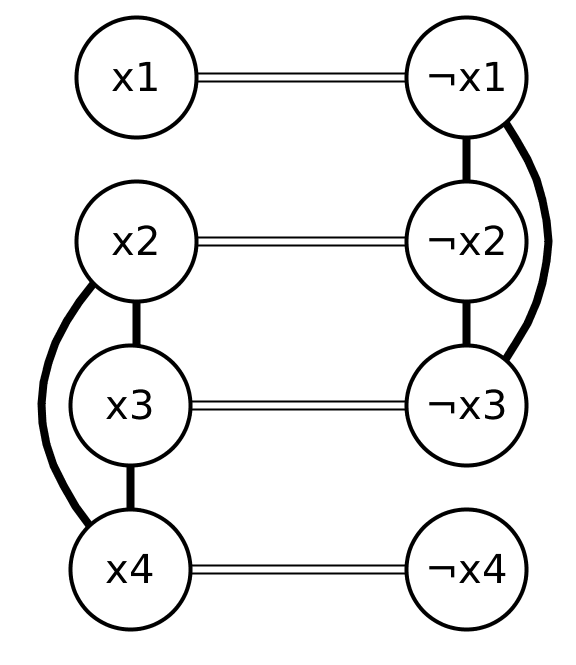
\includegraphics[width=6cm]{graph.png}
  \end{center}
  \caption{A conflict graph for constraints \ref{eq:1} and \ref{eq:2}.}
  \label{graph}
\end{figure}

Figure \ref{graph} shows the conflict graph for this constraints, where $\neg xi$ represents the complement (or deactivation) of variable $xi$. Initially, we create a vertex for each variable and its complement. Since in a feasible solution we can either activate a variable or its complement, we insert a edge between them (double lines). For constraint \ref{eq:1}, we have to transform it in a $\leq$-constraint, multiplying by -1. So, we have:

\[ - x_1 - x_2 - x_3 \leq - 2 \]

How the coefficients of this constraints are ordered, we can start calculating $L_{\ref{eq:1}}^{x_{\hat{j}}=1,\, x_{\hat{j}+1}=1}$. For any pair of activated variables we are able to produce a solution that respects this constraint. For this reason we do not find a clique with active variables in this constraint. Calculating $L_{\ref{eq:1}}^{x_{\hat{j}}=0,\, x_{\hat{j}+1}=0}$ for the first pair of subsequent variables (i.e. $\hat{j}=1$) we find a conflict that implies in a clique involving all complement of the variables starting from $x_1$ until $x_3$ ($L_{\ref{eq:1}}^{x_1=0,\, x_2=0} = -1$). So, we insert this conflicts in the graph.

We proceed analyzing constraint \ref{eq:2}. For any pair of deactivated variables we are able to produce a solution that respects this constraint. For this reason we do not find a clique with deactivated variables in this constraint. Calculating $L_{\ref{eq:2}}^{x_{\hat{j}}=1,\, x_{\hat{j}+1}=1}$ for the consecutive pairs of variables we can found a clique starting from $x_2$ until $x_4$ ($L_{\ref{eq:2}}^{x_{2}=1,\, x_{3}=1} = 5$). We finish inserting this conflicts in the graph.

\end{example}


\section{Clique Cut Separation}\label{cut}
\section{Experimental Results}\label{experiments}
\section{Conclusions and Future Work}\label{conclusions}

\bibliographystyle{endm}
\bibliography{references}

\end{document}
